\subsection{Recopilaci\'on final de datos del software para el informe 3}
    Se mape\'o una parte correspondiente a los edificios pertenecientes a la Escuela
        Superior de C\'omputo, perteneciente al Instituto Polit\'ecnico Nacional, en el cual se
        gener\'o una ruta la cual el robot deb\'ia de seguir para poder llegar desde un sal\'on a otro.
        Esta prueba de crucial, debido a que es realizada en un entorno que, a pesar de que en
        el mapa no es del todo claro, representa un reto debido a que en la vida real hay mucha
        gente la cual pasar\'a cerca del robot y podr\'ia implicar cierto riesgo a la hora de que el
        robot realice su trayecto, pudiendo llegar a ocasionar un accidente o posiblemente un
        fallo debido a la posible interferencia.
    \vskip 0.5cm
    %Figura
    \begin{figure}[h!]
        \centering
        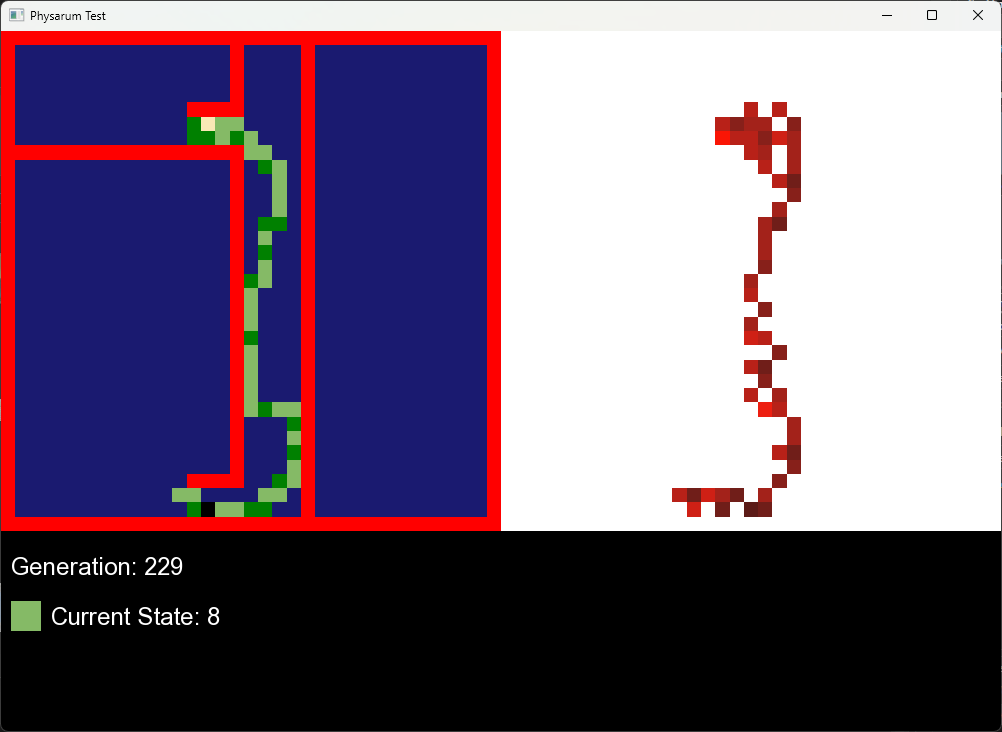
\includegraphics[width=0.8\textwidth]{./images/Pruebas/Imagen1.png}
        \caption{Esta es la ruta generada la cual el robot debe de seguir para poder llegar desde un sal\'on
            hasta el otro. La c\'elula negra representa el estado inicial y la c\'elula amarilla representa
            el destino final (nutriente encontrado).}
        \label{fig:Mapa_ESCOM}
    \end{figure}
    \vskip 0.5cm
    Como se puede observar en la Figura \ref{fig:Mapa_ESCOM}, la ruta generada por el algoritmo
        es la que se muestra en color verde, la cual es la ruta que el robot deber\'a de seguir para
        poder llegar desde el sal\'on 1 al sal\'on 2. Una vez generada la ruta, sus coordenadas fueron almacenadas y enviadas hacia el
        robot, el cual se encarg\'o de interpretarlas y as\'i seguir la ruta correspondiente a el mapa
        donde primeramente fue iniciada la simulaci\'on del Physarum. Esta ruta fue
        parcialmente corregida debido a las implicaciones que tiene el comportamiento
        natural del Physarum, en el cual, la ruta encontrada no necesariamente es de las
        mejores que se pueden obtener, debido al comportamiento del plasmodio que tiene
        de manera intr\'inseca
    \vskip 0.5cm
    %Figura
    \begin{figure}[h!]
        \centering
        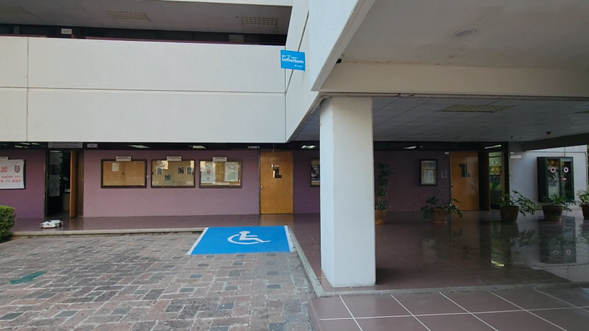
\includegraphics[width=0.8\textwidth]{./images/Pruebas/Imagen2.png}
        \caption{Robot saliendo del sal\'on 1 y siguiendo la ruta generada por el algoritmo del Physarum.}
        \label{fig:Mapa_ESCOM_Robot}
    \end{figure}
    \vskip 0.5cm
    \begin{figure}[h!]
        \centering
        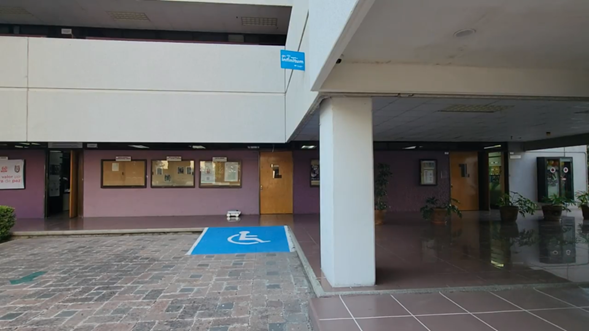
\includegraphics[width=0.8\textwidth]{./images/Pruebas/Imagen3.png}
        \caption{Robot a mitad de camino siguiendo la ruta generada por el algoritmo del Physarum.}
        \label{fig:Mapa_ESCOM_Robot2}
    \end{figure}
    \vskip 0.5cm
    \begin{figure}[h!]
        \centering
        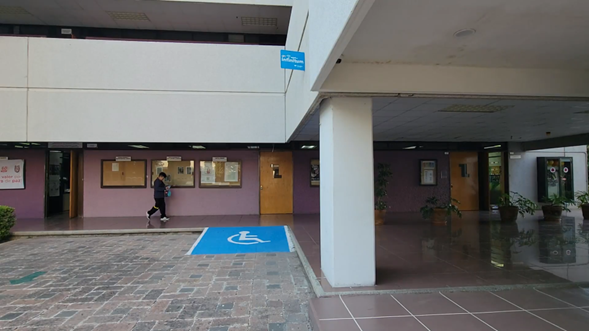
\includegraphics[width=0.8\textwidth]{./images/Pruebas/Imagen4.png}
        \caption{Robot llegando al destino final siguiendo la ruta generada por el algoritmo del Physarum.}
        \label{fig:Mapa_ESCOM_Robot3}
    \end{figure}
    \vskip 0.5cm
    Como se puede observar en las Figuras \ref{fig:Mapa_ESCOM_Robot} - \ref{fig:Mapa_ESCOM_Robot3}, 
        el robot sigue la ruta entre los dos salones, mostrando as\'i
        c\'omo es que el algoritmo ha generado la ruta completamente, as\'i tambi\'en mostrando
        el comportamiento del robot mientras sigue la ruta, en el cual constantemente se esta
        monitoreando para evitar cualquier incidente con las personas que recorren el lugar.
    \vskip 0.5cm
    As\'i podemos decir que las pruebas realizadas fueron satisfactorias, y los datos
        recopilados muestran que el comportamiento del robot es el esperado, por lo que esta
        y m\'as informaci\'on nos representan una gran \'area de mejora para los respectivos casos
        en los cuales podamos mapear diferentes tipos de lugares y locaciones con incluso
        m\'as informaci\'on la cual pueda representar un mayor reto para el robot.